% Created 2020-04-25 六 09:32
% Intended LaTeX compiler: pdflatex
\documentclass[11pt]{article}
\usepackage[utf8]{inputenc}
\usepackage[T1]{fontenc}
\usepackage{graphicx}
\usepackage{grffile}
\usepackage{longtable}
\usepackage{wrapfig}
\usepackage{rotating}
\usepackage[normalem]{ulem}
\usepackage{amsmath}
\usepackage{textcomp}
\usepackage{amssymb}
\usepackage{capt-of}
\usepackage{imakeidx}
\usepackage{hyperref}
\usepackage{minted}
% TIPS
% \substack{a\\b} for multiple lines text





% pdfplots will load xolor automatically without option
\usepackage[dvipsnames]{xcolor}

\usepackage{forest}
% two-line text in node by [two \\ lines]
% \begin{forest} qtree, [..] \end{forest}
\forestset{
  qtree/.style={
    baseline,
    for tree={
      parent anchor=south,
      child anchor=north,
      align=center,
      inner sep=1pt,
    }}}
%\usepackage{flexisym}
% load order of mathtools and mathabx, otherwise conflict overbrace

\usepackage{mathtools}
%\usepackage{fourier}
\usepackage{pgfplots}
\usepackage{amsthm}
\usepackage{amsmath}
%\usepackage{unicode-math}
%
\usepackage{commath}
%\usepackage{,  , }
\usepackage{amsfonts}
\usepackage{amssymb}
% importing symbols https://tex.stackexchange.com/questions/14386/importing-a-single-symbol-from-a-different-font
%mathabx change every symbol
% use instead stmaryrd
%\usepackage{mathabx}
\usepackage{stmaryrd}
\usepackage{empheq}
\usepackage{tikz}
\usepackage{tikz-cd}
%\usepackage[notextcomp]{stix}
\usetikzlibrary{arrows.meta}
\usepackage[most]{tcolorbox}
%\utilde
%\usepackage{../../latexpackage/undertilde/undertilde}
% left and right superscript and subscript
\usepackage{actuarialsymbol}
\usepackage{threeparttable}
\usepackage{scalerel,stackengine}
\usepackage{stackrel}
% \stackrel[a]{b}{c}
\usepackage{dsfont}
% text font
\usepackage{newpxtext}
%\usepackage{newpxmath}

%\newcounter{dummy} \numberwithin{dummy}{section}
\newtheorem{dummy}{dummy}[section]
\theoremstyle{definition}
\newtheorem{definition}[dummy]{Definition}
\newtheorem{corollary}[dummy]{Corollary}
\newtheorem{lemma}[dummy]{Lemma}
\newtheorem{proposition}[dummy]{Proposition}
\newtheorem{theorem}[dummy]{Theorem}
\theoremstyle{definition}
\newtheorem{example}[dummy]{Example}
\theoremstyle{remark}
\newtheorem*{remark}{Remark}


\newcommand\what[1]{\ThisStyle{%
    \setbox0=\hbox{$\SavedStyle#1$}%
    \stackengine{-1.0\ht0+.5pt}{$\SavedStyle#1$}{%
      \stretchto{\scaleto{\SavedStyle\mkern.15mu\char'136}{2.6\wd0}}{1.4\ht0}%
    }{O}{c}{F}{T}{S}%
  }
}

\newcommand\wtilde[1]{\ThisStyle{%
    \setbox0=\hbox{$\SavedStyle#1$}%
    \stackengine{-.1\LMpt}{$\SavedStyle#1$}{%
      \stretchto{\scaleto{\SavedStyle\mkern.2mu\AC}{.5150\wd0}}{.6\ht0}%
    }{O}{c}{F}{T}{S}%
  }
}

\newcommand\wbar[1]{\ThisStyle{%
    \setbox0=\hbox{$\SavedStyle#1$}%
    \stackengine{.5pt+\LMpt}{$\SavedStyle#1$}{%
      \rule{\wd0}{\dimexpr.3\LMpt+.3pt}%
    }{O}{c}{F}{T}{S}%
  }
}

\newcommand{\bl}[1] {\boldsymbol{#1}}
\newcommand{\Wt}[1] {\stackrel{\sim}{\smash{#1}\rule{0pt}{1.1ex}}}
\newcommand{\wt}[1] {\widetilde{#1}}
\newcommand{\tf}[1] {\textbf{#1}}


%For boxed texts in align, use Aboxed{}
%otherwise use boxed{}

\DeclareMathSymbol{\widehatsym}{\mathord}{largesymbols}{"62}
\newcommand\lowerwidehatsym{%
  \text{\smash{\raisebox{-1.3ex}{%
    $\widehatsym$}}}}
\newcommand\fixwidehat[1]{%
  \mathchoice
    {\accentset{\displaystyle\lowerwidehatsym}{#1}}
    {\accentset{\textstyle\lowerwidehatsym}{#1}}
    {\accentset{\scriptstyle\lowerwidehatsym}{#1}}
    {\accentset{\scriptscriptstyle\lowerwidehatsym}{#1}}
}

\usepackage{graphicx}
    
% text on arrow for xRightarrow
\makeatletter
%\newcommand{\xRightarrow}[2][]{\ext@arrow 0359\Rightarrowfill@{#1}{#2}}
\makeatother


\newcommand{\dom}[1]{%
\mathrm{dom}{(#1)}
}

% Roman numerals
\makeatletter
\newcommand*{\rom}[1]{\expandafter\@slowromancap\romannumeral #1@}
\makeatother

\def \fR {\mathfrak{R}}
\def \bx {\boldsymbol{x}}
\def \bz {\boldsymbol{z}}
\def \ba {\boldsymbol{a}}
\def \bh {\boldsymbol{h}}
\def \bo {\boldsymbol{o}}
\def \bU {\boldsymbol{U}}
\def \bc {\boldsymbol{c}}
\def \bV {\boldsymbol{V}}
\def \bI {\boldsymbol{I}}
\def \bK {\boldsymbol{K}}
\def \bt {\boldsymbol{t}}
\def \bb {\boldsymbol{b}}
\def \bA {\boldsymbol{A}}
\def \bX {\boldsymbol{X}}
\def \bu {\boldsymbol{u}}
\def \bS {\boldsymbol{S}}
\def \bZ {\boldsymbol{Z}}
\def \bz {\boldsymbol{z}}
\def \by {\boldsymbol{y}}
\def \bw {\boldsymbol{w}}
\def \bT {\boldsymbol{T}}
\def \bF {\boldsymbol{F}}
\def \bS {\boldsymbol{S}}
\def \bm {\boldsymbol{m}}
\def \bW {\boldsymbol{W}}
\def \bR {\boldsymbol{R}}
\def \bQ {\boldsymbol{Q}}
\def \bS {\boldsymbol{S}}
\def \bP {\boldsymbol{P}}
\def \bT {\boldsymbol{T}}
\def \bY {\boldsymbol{Y}}
\def \bH {\boldsymbol{H}}
\def \bB {\boldsymbol{B}}
\def \blambda {\boldsymbol{\lambda}}
\def \bPhi {\boldsymbol{\Phi}}
\def \btheta {\boldsymbol{\theta}}
\def \bTheta {\boldsymbol{\Theta}}
\def \bmu {\boldsymbol{\mu}}
\def \bphi {\boldsymbol{\phi}}
\def \bSigma {\boldsymbol{\Sigma}}
\def \lb {\left\{}
\def \rb {\right\}}
\def \la {\langle}
\def \ra {\rangle}
\def \caln {\mathcal{N}}
\def \dissum {\displaystyle\Sigma}
\def \dispro {\displaystyle\prod}
\def \E {\mathbb{E}}
\def \Q {\mathbb{Q}}
\def \N {\mathbb{N}}
\def \V {\mathbb{V}}
\def \R {\mathbb{R}}
\def \P {\mathbb{P}}
\def \A {\mathbb{A}}
\def \Z {\mathbb{Z}}
\def \I {\mathbb{I}}
\def \C {\mathbb{C}}
\def \cala {\mathcal{A}}
\def \calb {\mathcal{B}}
\def \calq {\mathcal{Q}}
\def \calp {\mathcal{P}}
\def \cals {\mathcal{S}}
\def \calg {\mathcal{G}}
\def \caln {\mathcal{N}}
\def \calr {\mathcal{R}}
\def \calm {\mathcal{M}}
\def \calc {\mathcal{C}}
\def \calf {\mathcal{F}}
\def \calk {\mathcal{K}}
\def \call {\mathcal{L}}
\def \calu {\mathcal{U}}
\def \bcup {\bigcup}


\def \uin {\underline{\in}}
\def \oin {\overline{\in}}
\def \uR {\underline{R}}
\def \oR {\overline{R}}
\def \uP {\underline{P}}
\def \oP {\overline{P}}

\def \Ra {\Rightarrow}

\def \e {\enspace}

\def \sgn {\operatorname{sgn}}
\def \gen {\operatorname{gen}}
\def \ker {\operatorname{ker}}
\def \im {\operatorname{im}}

\def \tril {\triangleleft}

% \varprod
\DeclareSymbolFont{largesymbolsA}{U}{txexa}{m}{n}
\DeclareMathSymbol{\varprod}{\mathop}{largesymbolsA}{16}

% \bigtimes
\DeclareFontFamily{U}{mathx}{\hyphenchar\font45}
\DeclareFontShape{U}{mathx}{m}{n}{
      <5> <6> <7> <8> <9> <10>
      <10.95> <12> <14.4> <17.28> <20.74> <24.88>
      mathx10
      }{}
\DeclareSymbolFont{mathx}{U}{mathx}{m}{n}
\DeclareMathSymbol{\bigtimes}{1}{mathx}{"91}
% \odiv
\DeclareFontFamily{U}{matha}{\hyphenchar\font45}
\DeclareFontShape{U}{matha}{m}{n}{
      <5> <6> <7> <8> <9> <10> gen * matha
      <10.95> matha10 <12> <14.4> <17.28> <20.74> <24.88> matha12
      }{}
\DeclareSymbolFont{matha}{U}{matha}{m}{n}
\DeclareMathSymbol{\odiv}         {2}{matha}{"63}


\newcommand\subsetsim{\mathrel{%
  \ooalign{\raise0.2ex\hbox{\scalebox{0.9}{$\subset$}}\cr\hidewidth\raise-0.85ex\hbox{\scalebox{0.9}{$\sim$}}\hidewidth\cr}}}
\newcommand\simsubset{\mathrel{%
  \ooalign{\raise-0.2ex\hbox{\scalebox{0.9}{$\subset$}}\cr\hidewidth\raise0.75ex\hbox{\scalebox{0.9}{$\sim$}}\hidewidth\cr}}}

\newcommand\simsubsetsim{\mathrel{%
  \ooalign{\raise0ex\hbox{\scalebox{0.8}{$\subset$}}\cr\hidewidth\raise1ex\hbox{\scalebox{0.75}{$\sim$}}\hidewidth\cr\raise-0.95ex\hbox{\scalebox{0.8}{$\sim$}}\cr\hidewidth}}}
\newcommand{\stcomp}[1]{{#1}^{\mathsf{c}}}


\author{Achim Klenke}
\date{\today}
\title{\aunclfamily\Huge Probability Theory\\ A \\Comprehensive Course}
\hypersetup{
 pdfauthor={Achim Klenke},
 pdftitle={\aunclfamily\Huge Probability Theory\\ A \\Comprehensive Course},
 pdfkeywords={},
 pdfsubject={},
 pdfcreator={Emacs 26.3 (Org mode 9.3.6)}, 
 pdflang={English}}
\begin{document}

\maketitle \clearpage
\tableofcontents \clearpage\section{Basic Measure Theory}
\label{sec:orgcf3b0c5}
\subsection{Classes of Sets}
\label{sec:orgf987b47}
\begin{definition}[]
A class of sets \(\cala\) is called
\begin{itemize}
\item \textbf{\(\cap\)-closed} or a \textbf{\(\pi\)-system} if \(A\cap B\in\cala\) whenever \(A,B\in\cala\)
\item \textbf{\(\sigma\text{-}\cap\)-closed} (closed under countable intersection)
\item \textbf{\(\cup\)-closed} (closed under unions)
\item \textbf{\(\sigma\text{-}\cup\)-closed}
\item \textbf{\textbackslash-closed}
\item closed under complements
\end{itemize}
\end{definition}

\begin{definition}[$\sigma$-algebra]
A class of sets \(\cala\subset 2^{\Omega}\) is called a \textbf{\(\sigma\)-algebra} if it
fullills the following three conditions
\begin{enumerate}
\item \(\Omega\in\cala\)
\item \(\cala\) is closed under complements
\item \(\cala\) is closed under countable unions
\end{enumerate}
\end{definition}


\begin{theorem}[]
If \(\cala\) is closed under complements, then we have the equivalence
\begin{align*}
\cala\text{ is }\cap\text{-closed}\quad&\Longleftrightarrow\quad\cala\text{ is }
\cup\text{-closed}\\
\cala\text{ is }\sigma\text{-}\cap\text{-closed}\quad&\Longleftrightarrow\quad\cala\text{ is }
\sigma\text{-}\cup\text{-closed}
\end{align*}
\end{theorem}

\begin{theorem}[]
\label{thm1.4}
Assume that \(\cala\) is \textbackslash-closed. Then the following statements hold:
\begin{enumerate}
\item \(\cala\) is \(\cup\)-closed
\item If in addition \(\cala\) is \(\sigma\text{-}\cup\)-closed, then \(\cala\) is 
\(\sigma\text{-}\cup\)-closed
\item Any countable (repectively finite) union of sets in \(\cala\) can be
expressed as a countable (respectively finite) disjoint union of sets in \(\cala\)
\end{enumerate}
\end{theorem}

\begin{proof}
\begin{enumerate}
\setcounter{enumi}{2}
\item Assume that \(A_1,A_2,\dots\in\cala\)
\begin{equation*}
\displaystyle\bigcup_{n=1}^\infty A_n=A_1\uplus(A_2\textbackslash
A_1)\uplus((A_3\textbackslash
A_2)\textbackslash A_1)\uplus\dots
\end{equation*}
\end{enumerate}
\end{proof}

\begin{definition}[]
A class of sets \(\cala\subset 2^\Omega\) is called an \textbf{algebra} if the
following three conditions are fulfilled
\begin{enumerate}
\item \(\Omega\in\cala\)
\item \(\cala\) is \textbackslash-closed
\item \(\cala\) is \(\cup\)-closed
\end{enumerate}
\end{definition}

\begin{theorem}[]
A class of sets \(\cala\subset2^\Omega\) is an algebra if and only if the
following  three properties hold
\begin{enumerate}
\item \(\Omega\in\cala\)
\item \(\cala\) is closed under complements
\item \(\cala\) is closed under intersections
\end{enumerate}
\end{theorem}

\begin{definition}[]
A class of sets \(\cala\subset2^\Omega\) is called a \textbf{ring} if the following
conditions hold
\begin{enumerate}
\item \(\emptyset\in\cala\)
\item \(\cala\) is \textbackslash-closed
\item \(\cala\) is \(\cup\)-closed
\end{enumerate}
\end{definition}


\begin{definition}[]
A class of sets \(\cala\subset2^\Omega\) is called a \textbf{semiring} if
\begin{enumerate}
\item \(\emptyset\in\cala\)
\item for any two sets \(A,B\in\cala\) the difference set \(B\textbackslash A\) is a
finite union of mutually disjoint sets in \(\cala\)
\item \(\cala\) is \(\cap\)-closed
\end{enumerate}
\end{definition}

\begin{definition}[]
A class of sets \(\cala\subset2^\Omega\) is called a \textbf{\(\lambda\)-system} if
\begin{enumerate}
\item \(\Omega\in\cala\)
\item for any two sets \(A,B\in\cala\) with \(A\subset B\), \(B\textbackslash A\in\cala\)
\item \(\biguplus_{n=1}^\infty A_n\in\cala\) for any choice of countably many
pairwise disjoint sets \(A_1,\dots\in\cala\)
\end{enumerate}
\end{definition}

\begin{theorem}[]
\begin{enumerate}
\item Every \(\sigma\)-algebra also is a \(\lambda\)-system, an algebra and a
\(\sigma\)-ring
\item Every \(\sigma\)-ring is a ring, and every ring is a semiring
\item Every algebra is a ring. An algebra on a finite set \(\Omega\) is a \(\sigma\)-algebra
\end{enumerate}
\end{theorem}

\begin{definition}[liminf and limsup]
Let \(A_1,A_2,\dots\) be a subset of \(\Omega\). The sets
\begin{equation*}
\liminf_{n\to\infty}A_n:=\displaystyle\bigcup_{n=1}^\infty
\bigcap_{m=n}^\infty A_m\hspace{1.5cm}
\limsup_{n\to\infty}A_n:=\bigcap_{n=1}^\infty\bigcup_{m=n}^\infty
A_m
\end{equation*}
are called \textbf{limes inferior} and \textbf{limes superior}, respectively, of the sequence
\((A_n)_{n\in\N}\)
\end{definition}

\begin{remark}
\begin{enumerate}
\item lim\hspace{0.03cm}inf and lim\hspace{0.03cm}sup can be rewritten as
\begin{align*}
\liminf_{n\to\infty}A_n&=\{\omega\in\Omega:\#\{n\in\N:\omega\not\in A_n\}<\infty\}\\
\limsup_{n\to\infty}A_n&=\{\omega\in\Omega:\#\{n\in\N:\omega\in A_n\}=\infty\}
\end{align*}
In other words, limes inferior is the event where \textbf{eventually all} of the
\(A_n\) occur. On the other hand, limes superior is the event where
\textbf{infinitely many} of the \(A_n\) occur. In particular,
\(A_*:=\liminf_{n\to\infty}A_n\subset A^*:=\limsup_{n\to\infty}A_n\)
\item We define the \textbf{indicator function} on the set \(A\) by
\begin{equation*}
\mathbbm{1}_A(x):=
\begin{cases}
1,&x\in A\\
0,&x\not\in A
\end{cases}
\end{equation*}
With this notation 
\begin{equation*}
\mathbbm{1}_{A_*}=\liminf_{n\to\infty}\mathbbm{1}_{A_n}\quad\text{and}\quad
\mathbbm{1}_{A^*}=\limsup_{n\to\infty}\mathbbm{1}_{A_n}
\end{equation*}
\item If \(\cala\subset2^\Omega\) is a \(\sigma\)-algebra and if \(A_n\in\cala\) for
every \(n\in\N\), then \(A_*\in\cala\) and \(A^*\in\cala\)
\end{enumerate}
\end{remark}

\begin{theorem}[Intersection of classes of sets]
Let \(I\) be an arbitrary index set, and assume that \(\cala_i\) is a
\(\sigma\)-algebra for every \(i\in I\). Hence the intersection
\begin{equation*}
\cala_I:=\{A\subset\Omega:A\in\cala_i\text{ for every }i\in I\}=
\displaystyle\bigcap_{i\in I}\cala_i
\end{equation*}
is a \(\sigma\)-algebra. The analogous statement holds for rings, \(\sigma\)-rings,
algebras and \(\lambda\)-systems. However, it fails for semirings
\end{theorem}

\begin{theorem}[Generated $\sigma$-algebra]
Let \(\cale\subset2^\Omega\). Then there exists a smallest \(\sigma\)-algebra 
\(\sigma(\cale)\) with \(\cale\subset\sigma(\cale)\)
\begin{equation*}
\sigma(\cale):=\displaystyle\bigcap_{\substack{\cala\subset2^\Omega
\text{ is a }\sigma\text{-algebra}\\\cala\supset\cale}}\cala
\end{equation*}
\(\sigma(\cale)\) is called the \(\sigma\)-algebra generated by \(\cale\). \(\cale\) is
called a generator of \(\sigma(\cale)\). Similarly, we define \(\delta(\cale)\)
as the \(\lambda\)-system generated by \(\cale\)
\end{theorem}

\begin{remark}
The following three statements hold 
\begin{enumerate}
\item \(\cale\subset\sigma(\cale)\)
\item If \(\cale_1\subset\cale_2\), then \(\sigma(\cale_1)\subset\sigma(\cale_2)\)
\item \(\cala\) is a \(\sigma\)-algebra if and only if \(\sigma(\cala)=\cala\)
\end{enumerate}
\end{remark}

\begin{theorem}[$\cap$-closed $\lambda$-system]
\label{thm1.18}
Let \(\cald\subset2^\Omega\) be a \(\lambda\)-system. Then 
\begin{equation*}
\cald\text{ is a }\pi\text{-system}\quad\Longleftrightarrow\quad
\cald\text{ is a }\sigma\text{-algebra}
\end{equation*}
\end{theorem}

\begin{proof}
"\(\Longrightarrow\)"
\begin{enumerate}
\setcounter{enumi}{2}
\item Let \(A,B\in\cald\). By assumption, \(A\cap B\in\cald\) and trivially
\(A\cap B\subset A\). Thus \(A\textbackslash B=A\textbackslash(A\cap
      B)\in\cald\). This implies that \(\cald\) is \textbackslash-closed. Thus by
Theorem \ref{thm1.4}, works.
\end{enumerate}
\end{proof}


\begin{theorem}[Dynkin's $\pi$-$\lambda$ theorem]
If \(\cale\subset2^\Omega\) is a \(\pi\)-system, then
\begin{equation*}
\sigma(\cale)=\delta(\cale)
\end{equation*}
\end{theorem}

\begin{proof}
\begin{enumerate}
\item \(\supseteq\). \(A^c=\Omega\textbackslash A\).
\item \(\subseteq\). By Theorem \ref{thm1.18}, it is enough to show that
\(\delta(\cale)\) is a \(\pi\)-system. For any \(B\in\delta(\cale)\) define
\begin{equation*}
\cald_B:=\{A\in\delta(\cale):A\cap B\in\delta(\cale)\}
\end{equation*}
In order to show that \(\delta(\cale)\) is a \(\pi\) system, it is enough to
show that 
\begin{equation*}
\delta(\cale)\subset\cald_B\quad\text{for any }B\in\delta(\cale)
\end{equation*}

\(\cald_E\) is a \(\lambda\)-system
\begin{enumerate}
\item \(\Omega\cap E=E\in\delta(\cale)\). Hence \(\Omega\in\cald_E\)
\item For any \(A,B\in\cald_E\) with \(A\subset B\), we have 
\((B\textbackslash A)\cap E=(B\cap E)\textbackslash(A\cap E)\in\delta(E)\)
\item Assume that \(A_1,\dots,\in\cald_E\) are mutually disjoint. Hence
\begin{equation*}
\left(\displaystyle\bigcup_{n=1}^\infty\right)\cap E=
\biguplus_{n=1}^\infty(A_n\cap E)\in\delta(\cale)
\end{equation*}
\end{enumerate}
\end{enumerate}


By assumption, \(A\cap E\in\cale\) if \(A,E\in\cale\); thus
\(\cale\subset\cale_E\) if \(E\in\cale\). Hence
\(\delta(\cale)\subset\delta(\cald_E)=\cald_E\) for any \(E\in\cale\). Hence we
get that \(B\cap E\in\delta(\cale)\) for any \(B\in\delta(\cale)\) and
\(E\in\cale\). This implies that \(E\in\cale_B\) for any
\(B\in\delta(\cale)\). Thus \(\cale\subset\cald_B\) for any
\(B\in\delta(\cale)\). 
\end{proof}

\begin{figure}[htbp]
\centering
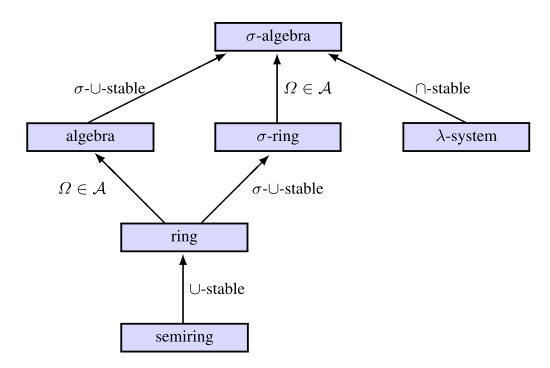
\includegraphics[width=.9\linewidth]{/media/wu/file/stuuudy/notes/images/ProbabilityTheory/classes.png}
\caption{\label{fig:org87f1637}Inclusions between classes of sets \(\cale\subset2^\Omega\)}
\end{figure}

\begin{definition}[Topology]
Let \(\Omega\neq\emptyset\) be an arbitrary set. A class of sets
\(\tau\subset2^\Omega\) is called a \textbf{topology} if it has the following three
properties:
\begin{enumerate}
\item \(\emptyset,\Omega\in\tau\)
\item \(A\cap B\in\tau\) for any \(A,B\in\tau\)
\item \(\bigcup_{A\in\calf}A\in\tau\) for any \(\calf\subset\tau\)
\end{enumerate}
\end{definition}

The pair \((\Omega,\tau)\) is called a \textbf{topological space}. The sets \(A\in\tau\) are
called \textbf{open}, and the sets \(A\subset\Omega\) with \(A^c\in\tau\) are called closed

Let \(d\) be a metric on \(\Omega\), and denote the open ball with radius \(r>0\)
centered at \(x\in\Omega\) by
\begin{equation*}
 B_r(x)=\{y\in\Omega:d(x,y)<r\}
\end{equation*}
Then the usual class of open sets is the topology
\begin{equation*}
\tau=\left\{\displaystyle\bigcup_{(x,r)\in F}B_r(x):F\subset\Omega
\times(0,\infty)\right\}
\end{equation*}



\begin{definition}[Borel \(\sigma\)-algebra]
Let \((\Omega,\tau)\) be a topological space. The \(\sigma\)-algebra 
\begin{equation*}
\calb(\Omega):=\calb(\Omega,\tau):=\sigma(\tau)
\end{equation*}
that is generated by the open sets is called the \textbf{Borel \(\sigma\)-algebra} on
\(\Omega\). The elements \(A\in\calb(\Omega,\tau)\) are called \textbf{Borel sets} or \textbf{Borel measuable sets}
\end{definition}




For \(a,b\in\R^n\), we write 
\begin{equation*}
a<b\quad\text{if }a_i<b_i\quad\text{for all }i=1,\dots,n
\end{equation*}
For \(a<b\), we define the open \textbf{rectangle} as the Cartesian product
\begin{equation*}
(a,b):=\bigtimes_{i=1}^n(a_i,b_i):=(a_1,b_1)\times(a_2,b_2)\times\dots\times
(a_n,b_nx)
\end{equation*}

\begin{definition}[Trace of a class of sets]
Let \(\cala\subset2^\Omega\) be an arbitrary class of subsets of \(\Omega\) and let 
\(A\in2^\Omega\textbackslash\{\emptyset\}\). The class 
\begin{equation*}
\cala|_A:=\{A\cap B:B\in\cala\}\subset2^A
\end{equation*}
is called the \textbf{trace} of \(\cala\) on \(A\) or the \textbf{restriction} of \(\cala\) on \(A\)
\end{definition}

\begin{theorem}[]
Let \(A\subset\Omega\) be a nonempty set and let \(\cala\) be a
\(\sigma\)-algebra on \(\Omega\) (ring,semiring,). Then \(\cala|_A\)
is a class of sets of the same type as \(\cala\); however on \(A\) instead of \(\Omega\).
For \(\lambda\)-systems this is not true in general
\end{theorem}
\subsection{Set Functions}
\label{sec:org6008a8a}
\begin{definition}[]
Let \(\cala\subset2^\Omega\)  and let \(\mu:\cala\to[0,\infty]\) be a set
function. We say that \(\mu\) is 
\begin{enumerate}
\item \textbf{monotone} if \(\mu(A)\le\mu(B)\) for any two sets \(A,B\in\cala\) with
\(A\subset B\)
\item \textbf{additive} if \(\mu(\biguplus_{i=1}^n A_i)=\sum_{i=1}^n \mu(A_i)\) for any choice of
finitely many mutually disjoint sets \(A_1,\dots,A_n\in\cala\) with 
\(\bigcup_{i=1}^n A_i\in\cala\)
\item \textbf{\(\sigma\)-additive} if 
\(\mu(\biguplus_{i=1}^\infty A_i)=\sum_{i=1}^\infty \mu(A_i)\) for any choice of 
countably many mutually disjoint sets \(A_1,\dots\in\cala\) with 
\(\bigcup_{i=1}^\infty A_i\in\cala\)
\item \textbf{subadditive} if for any choice of finitely many sets
\(A,A_1,\dots,A_n\in\cala\) with \(A\subset\bigcup_{i=1}^nA_i\), we have
\(\mu(A)\le\sum_{i=1}^n\mu(A_i)\)
\item \textbf{\(\sigma\)subadditive} if for any choice of countably many sets
\(A,A_1,\dots\in\cala\) with \(A\subset\bigcup_{i=1}^\infty A_i\), we have
\(\mu(A)\le\sum_{i=1}^\infty\mu(A_i)\)
\end{enumerate}
\end{definition}

\begin{definition}[]
Let \(\cala\) be a semiring and let \(\mu:\cala\to[0,\infty]\) be a set function
with \(\mu(\emptyset)=0\), \(\mu\) is called a
\begin{itemize}
\item \textbf{content} if \(\mu\) is additive
\item \textbf{premeasure} if \(\mu\) is \(\sigma\)-additive
\item \textbf{measure} if \(\mu\) is a premeasure and \(\cala\) is a \(\sigma\)-algebra
\item \textbf{probability measure} if \(\mu\) is a measure and \(\mu(\Omega)=1\)
\end{itemize}
\end{definition}

\begin{definition}[]
Let \(\cala\) be a semiring. A content \(\mu\) on \(\cala\) is called
\begin{enumerate}
\item \textbf{finite} if \(\mu(A)<\infty\) for every \(A\in\cala\) and
\item \textbf{\(\sigma\)-finite} if there exists a sequence of sets
\(\Omega_1,\Omega_2,\dots,\in\cala\) s.t.
\(\Omega=\bigcup_{n=1}^\infty\Omega_n\) and s.t. \(\mu(\Omega_n)<\infty\)
for all \(n\in\N\)
\end{enumerate}
\end{definition}

\begin{examplle}[Contents, measures]
\begin{enumerate}
\item Let \(\omega\in\Omega\) and \(\delta_\omega(A)=\mathbbm{1}_A(\omega)\). Then
\(\delta_\omega\) is a probability measure on any \(\sigma\)-algebra 
\(\cala\subset2^\Omega\). \(\delta_\omega\) is called the \textbf{Dirac measure} for
the point \(\omega\)
\item Let \(\Omega\) be a finite nonempty set. By 
\begin{equation*}
\mu(A):=\frac{\#A}{\#B}\quad\text{for }A\subset\Omega
\end{equation*}
we define a probability measure on \(\cala=2^\Omega\). This \(\mu\) is called the
\textbf{uniform distribution} on \(\Omega\). For this distribution, we introduce the symbol
\(\calu_\Omega:=\mu\). The resulting triple \((\Omega,\cala,\calu_\Omega)\) is
called a \textbf{Laplace space}
\end{enumerate}
\end{examplle}

\begin{lemma}[Properties of contents]
Let \(\cala\) be a semiring and let \(\mu\) be a content on \(\cala\). Then the
following statements hold.
\begin{enumerate}
\item If \(\cala\) is a ring, then \(\mu(A\cup B)+\mu(A\cap B)=\mu(A)+\mu(B)\)
\item \(\mu\) is monotone. If \(\cala\) is a ring, then \(\mu(B)=\mu(A)+\mu(B\A)\) for
any two sets \(A,B\in\cala\) with \(A\subset B\)
\item \(\mu\) is subadditive. If \(\mu\) is \(\sigma\)-additive, then \(\mu\) is also \(\sigma\)-subadditive
\item If \(\cala\) is a ring then
\(\sum_{n=1}^\infty\mu(A_n)\le\mu(\bigcup_{n=1}^\infty A_n)\) for any
choice of countably many mutually disjoint sets \(A_1,\dots\in\cala\) with 
\(\bigcup_{n=1}^\infty A_n\in\cala\)
\end{enumerate}
\end{lemma}

\#+END\textsubscript{definition}
\end{document}